\documentclass[10pt]{article}
\usepackage[margin=0.7in]{geometry}
\usepackage[T1]{fontenc}
\usepackage[utf8]{inputenc}
\usepackage{graphicx}
\usepackage{caption}
\usepackage{subcaption}
\usepackage{booktabs}
\usepackage{tabularx}
\usepackage{multicol}
\usepackage{amsmath}
\usepackage{xcolor}

\setlength{\parindent}{0pt}
\setlength{\parskip}{4pt}

\begin{document}

\begin{center}
{\LARGE \textbf{Linear regression demonstration}}\\
\end{center}
\vspace{4pt}
\hrule
\vspace{10pt}

\textbf{Notes}\\

Synthetic dataset with Gaussian noise, ipsum lorem, ipsum lorem, ipsum lorem, ipsum lorem, ipsum lorem, ipsum lorem, ipsum lorem, ipsum lorem

\vspace{8pt}

\begin{figure}[h!]
    \centering
    \scalebox{1.0}[1.0]{%
        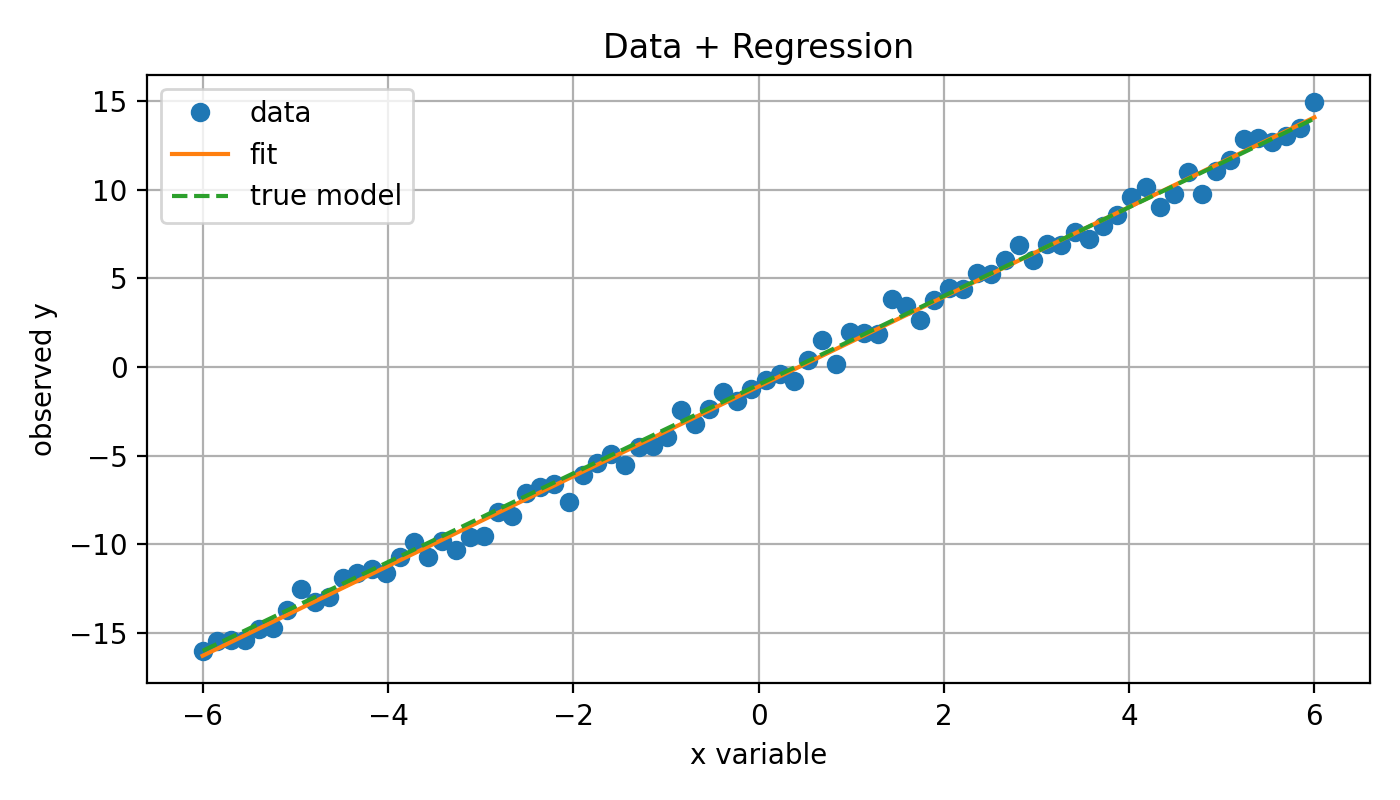
\includegraphics{plot_data_fit.png}%
    }
    \caption{Graph showing linear regression of Demo dataset + true model of Linear regression demonstration}
    \label{fig:placeholder}
\end{figure}

\begin{multicols}{2}

\textbf{Fit summary}\\[-2pt]
\begin{tabularx}{\linewidth}{@{}lX@{}}
\toprule
Key & Value \\
\midrule
Model & linear \\
$R^2$ & 0.9966 \\
RMSE & 0.5212 \\
$\chi^2$ & 60.37 \\
$\chi^2_{\mathrm{red}}$ & 0.7739 \\
dof & 78 \\
weighted & Yes \\
absolute sigma & Yes \\
method & None \\
maxfev & 100000 \\
bounds & Yes \\
initial guess p0 & (not stored) \\
\bottomrule
\end{tabularx}

\vspace{15pt}

\[
f(x) = 2.529 x - 1.106
\]

\columnbreak

\textbf{Fitted parameters}\\[-2pt]
\begin{tabularx}{\linewidth}{@{}lX@{}}
\toprule
Parameter & Estimate \\
\midrule
A & 2.529 $\pm$ 0.01912 \\
B & -1.106 $\pm$ 0.06708 \\
\bottomrule
\end{tabularx}

\vspace{8pt}

\textbf{Dataset info}\\[-0pt]
\vspace{2pt}
\begin{tabularx}{\linewidth}{@{}lX@{}}
\toprule
Key & Value \\
\midrule
Name & Demo dataset \\
n (samples) & 80 \\
d (features) & 1 \\
x label & x variable \\
y label & observed y \\
yerr & Provided \\
xerr & None \\
x min/max & x1: [-6, 6] \\
y min/max & [-16, 14.91] \\
\bottomrule
\end{tabularx}

\end{multicols}

\end{document}